\chapter{Experiments and Evaluations\label{cha:chapter4}}

To evaluate the Frankenbot's modular architecture on the basis of the user experience, the surveys has been conducted. 
\\~\\
For accomplishment of this research, random users were selected irrespective of their profession, studies background and any race or gender discrimination. But the age limit constraint was set to be above 18. As participants were considered to be accused of a robbery and have to chat with a detective bot and answer his questions which can be a bit rude and straight forward for youngsters below 18. So the participant with the minimum age was 22. On contrary, the one with the maximum age was 34. And the average age calculated as 25.65 with the standard deviation of 2.37. Visuals have been shown in the Figure \ref{fig:ageGraph}.

\begin{figure}[!h]
    \centering
    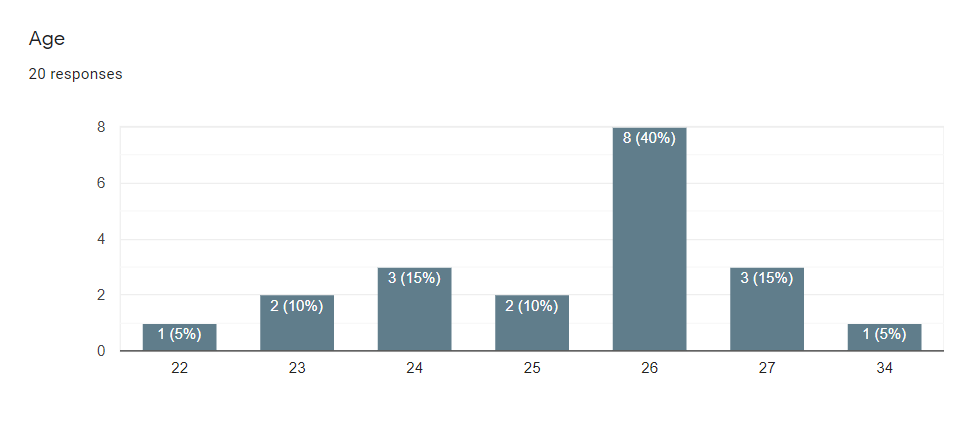
\includegraphics[width=0.9\textwidth]{img/Age_Graph.PNG}
    \caption{Age stats of participants}
    \label{fig:ageGraph}
\end{figure}
\\~\\
Total 20 users participated in this study. Most of them appeared to be from technical background as maximum of them were students from different universities. Secondly, majority of participants revealed themselves to be IT employees other than the students. While remaining revealed themselves as engineer, teacher and business qualified. More details have been shown in the Figure \ref{fig:profGraph}.

\begin{figure}[!h]
    \centering
    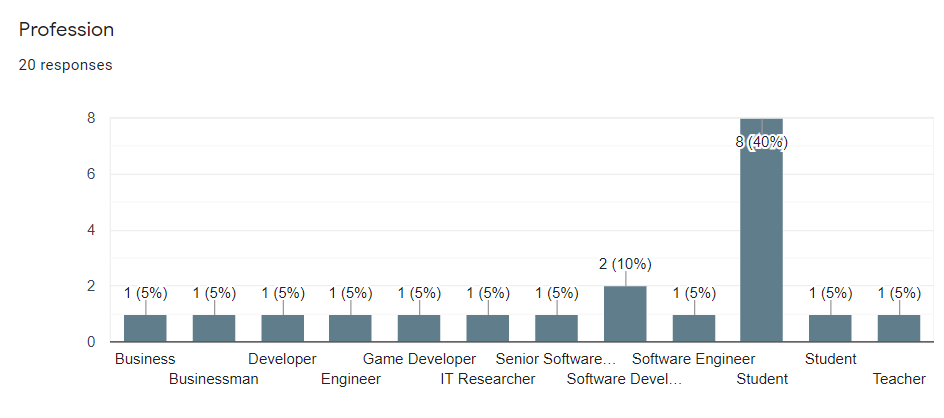
\includegraphics[width=0.9\textwidth]{img/Profession_Graph.PNG}
    \caption{Profession related details of participants}
    \label{fig:profGraph}
\end{figure}

\section{Experimental Setup}
This research study has been conducted to gather the results for what user has experienced while interacting with the chatbot. 
\\~\\
The users were asked to complete two surveys. One named as "Frankenbot's Experience Survey" was designed with the help of \cite{MOLLER200726}\cite{itut}. For the second survey, the standardized tool to personally evaluate the usability and design of an interactive product known as AttrakDiff\cite{attrakdiff} has been used. First survey was designed using Google Forms and the purpose of it was to capture the user's interaction experience about the Frankenbot. While, the purpose of AttrakDiff's study was to evaluate the Frankenbot's hedonic(joy of use, stimulation, identification) and pragmatic(usefulness, efficiency, easy to use) qualities. 
\\~\\
The users were provided with the link to the deployed chatbot's interface as a web page and they can easily access it from their own places. It provided ease to the user and enhanced the comfortability factor for them. Also, they have to read the description and instructions provided for them on the web page. And they have to figure out what to do and how to operate the chatbot on their own without any external help. Which has given more realistic and unbiased essence to the results obtained.
\\~\\
For the surveys, the web page contains the heading as "Frankenbot's Request" in which the users were requested to complete the surveys once, they are finished having chat for a fun purpose with the chatbot. They have been provided with the links to the surveys.
\\~\\
The surveys were conducted in English language. Whereas, AttrakDiff's survey has the option for both English and German. You can find the "Frankenbot's Experience Survey" in the Appendices \ref{appen:survey}. Furthermore, AttrakDiff's Individual Evaluation Study\cite{indeval} has been used as the second survey.
% \begin{enumerate}
%     \item 
%     \item max-activation-dialogue-manager; recall the same function with a json for each module in a list of modules and returns a class MaxActivationDialogueTreeManager's object afterwards.
%     \item dialogue-tree; recall the same function with a json for a dialogue tree and returns a tree consisting of tree nodes afterwards.
%      \item tree-node; recall the same function with a json for each element of a list dialogue tree and returns a class Atom's object afterwards.
%      \item simple-response-generator; recall the same function with a json for a response generator and returns a class SimpleResponseGenerator's object afterwards.
% \end{enumerate} 

